\section{The Continuous and Discrete Fourier Transforms}
\label{ch:11}

\textit{Summary}
\begin{itemize}
    \item This chapter is focused on the continuous and discrete Fourier Transforms relevant to MR imaging.

    \item In the absence of relaxation effects, $s(\vec{k})$ and $\rho(\vec{r})$ are \textbf{Fourier transform pairs}.

    \item The reconstructed image, $\hat{\rho}(\vec{r})$, represents an \textbf{estimate} of the \textbf{effective spin density} due to various \textbf{numerical approximations} that take place during the MR imaging process (from \textbf{discretised} and \textbf{truncated} signal sampling).    
\end{itemize}

\begin{figure}[H]
    \centering
    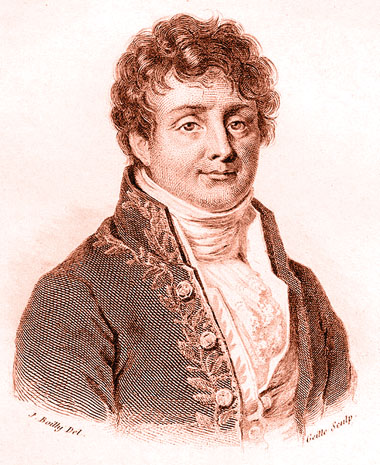
\includegraphics[width=.6\textwidth,keepaspectratio]{FourierJeanBaptiste}
    \caption{Jean-Baptiste Joseph Fourier \courtesywiki}
    \label{fig:FourierJeanBaptiste}
\end{figure}


\clearpage
%%
\subsection{The Continuous Fourier Transform}

\begin{itemize}

    \item The \textbf{Fourier transform is a functional}, mapping a function to another function. \\ \\
    Let: \\
    $h$ be a function of x-space (or time space) and \\
    $H$ be a function of k-space (or frequency space) then: \\
    \begin{flalign*}
        \mathfrak{F}      & : (h) \rightarrow (H) \\
        \mathfrak{F}^{-1} & : (H) \rightarrow (h)   \\
        \mathfrak{F} \circ \mathfrak{F}^{-1} & = \text{identity}
    \end{flalign*}

    In MRI, the \textbf{Fourier transform maps a function} from \textbf{position space (x-space)} to its \textbf{'conjugate' space (k-space)}, and back, through the inverse Fourier transform.

    \item Fourier Transform Pairs in MRI: $\rho(\vec{r}) \xLeftrightarrow{\mathfrak{F}} s(\vec{k})$, where \\
    $\rho(\vec{r})$ = \textbf{spin density in x-space (position space)} and \\
    $s(\vec{k})$ = \textbf{signal in k-space (spatial frequency space)}

    \item Knowing the \textbf{signal equation }: \\
    \begin{flalign*}
        s(\vec{k}) = \int_{- \infty}^{+ \infty} d\vec{r} \ \rho(\vec{r}) e^{-i 2 \pi \vec{k} \cdot \vec{r}}
    \end{flalign*}
    the \textbf{Fourier transform pairs} are shown for the general case: \\
    \begin{flalign*}
        H(\vec{k}) \equiv \mathfrak{F}(h(\vec{r})) & = \int_{- \infty}^{+ \infty} d\vec{r} \ h(\vec{r}) e^{-i 2 \pi \vec{k} \vec{r}} \\ 
        h(\vec{r}) \equiv \mathfrak{F}^{-1}(H(\vec{k})) & = \int_{- \infty}^{+ \infty} d\vec{k} \ H(\vec{k}) e^{+i 2 \pi \vec{k} \vec{r}} 
    \end{flalign*}
    and for \textbf{Dirac delta functions}, knowing from (Book 9.24) that $\delta(\vec{r}) = \int_{- \infty}^{+ \infty} d\vec{k} \ e^{i 2 \pi \vec{k} \cdot \vec{r}}$, we have:
    \begin{flalign*}
        \delta(\vec{k} - \vec{k}_0) & = \int_{- \infty}^{+ \infty} d\vec{r} \ e^{-i 2 \pi (\vec{k}-\vec{k}_0) \cdot \vec{r}} \\ 
        \delta(\vec{r} - \vec{r}_0) & = \int_{- \infty}^{+ \infty} d\vec{k} \ e^{+i 2 \pi \vec{k} \cdot (\vec{x}-\vec{x}_0) }
    \end{flalign*}
    
    \textcolor{gray}{\textbf{Sidenote}: $\delta(\vec{r}) \equiv \mathfrak{F}^{-1}(G(\vec{k})) = \int_{- \infty}^{+ \infty} d\vec{k} \ G(\vec{k}) \  e^{i 2 \pi \vec{k} \cdot \vec{r}} \Rightarrow G(\vec{k}) = 1$. This is very interesting as we have seen in Book Chapter 9.3.1, that $\delta(x) = \lim_{K\to\infty} 2K \ sinc(2 \pi K x)$ (see Figure~\ref{fig:figeq928}), which shows that, at the limit, the Dirac delta function encompasses all possible frequencies. Therefore, its Fourier transform will be a straight line.}
    
    \item The identity property ($\mathfrak{F} \circ \mathfrak{F}^{-1} = \text{identity}$) can be derived like this: \\
    \begin{flalign*}
        h(x) & = \int_{- \infty}^{+ \infty} dk \ H(k) e^{+i 2 \pi k x} \\
             & = \int_{- \infty}^{+ \infty} dk \ \int_{- \infty}^{+ \infty} dx' \ h(x') e^{-i 2 \pi k x'} \ \ e^{+i 2 \pi k x} \\
             & = \int_{- \infty}^{+ \infty} dx' \ h(x') \int_{- \infty}^{+ \infty} dk \ e^{+i 2 \pi k (x-x')} \\
             & = \int_{- \infty}^{+ \infty} dx' \ h(x') \delta(x-x') \text{ (See Book 9.27)}\\
             & = h(x)
    \end{flalign*}

    \item A continuous signal $s(k)$, known for all $k$, can be used to retrieve the \textbf{spin density} (Book 11.7): \\
    \begin{flalign*}
        \rho(\vec{r}) = \int_{- \infty}^{+ \infty} d\vec{k} \ s(\vec{k}) e^{+i 2 \pi \vec{k} \cdot \vec{r}}
    \end{flalign*}
    In fact, the signal is not known for all $k$, but it is an approximation of the continuous form. \\
    The actual signal is finitely sampled, it is called $s_m(k)$ (measured signal) and it yields the reconstructed image $\hat{\rho(x)}$ through a continuous inverse Fourier transform:
    \begin{flalign*}
        \hat{\rho}(\vec{r}) = \int_{- \infty}^{+ \infty} d\vec{k} \ s_m(\vec{k}) e^{+i 2 \pi \vec{k} \cdot \vec{r}}
    \end{flalign*}

    \item The differences between $\rho(\vec{r})$ and $\hat{\rho}(\vec{r})$ are very important in understanding imaging artifacts.
\end{itemize}

\begin{figure}[H]
    \centering
    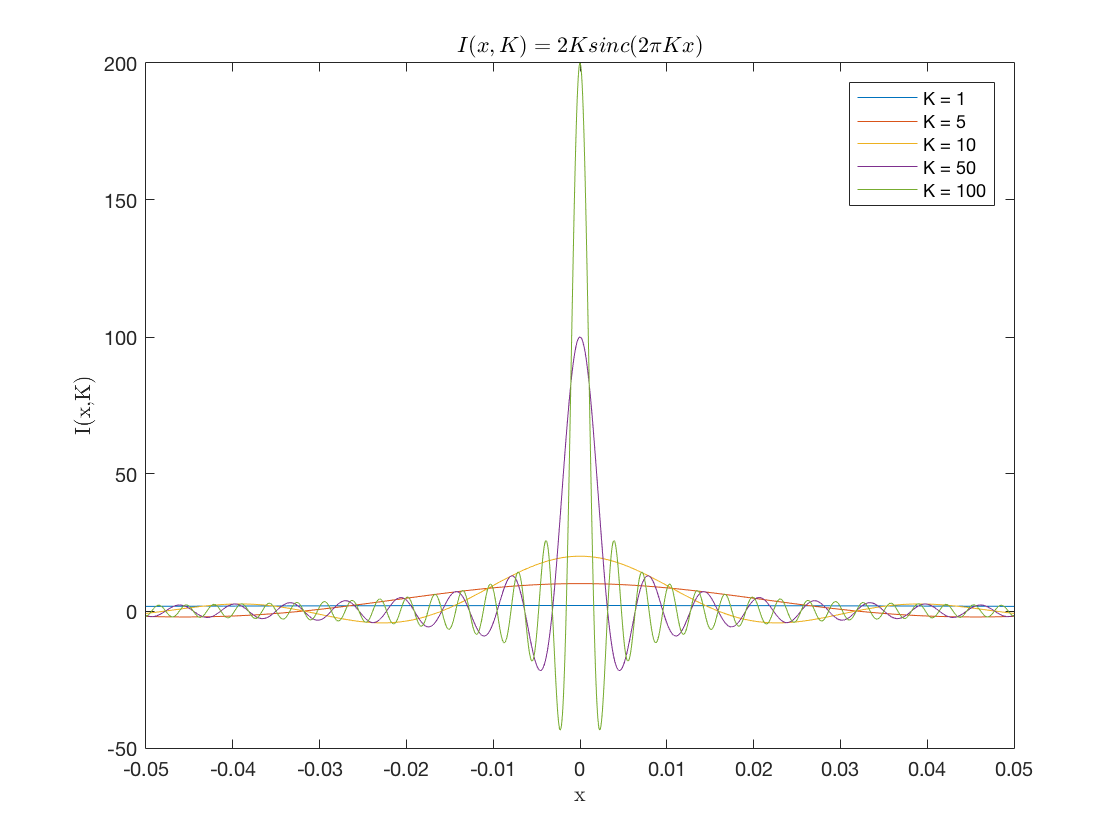
\includegraphics[width=.7\textwidth,keepaspectratio]{figeq928}
    \caption{When the $sinc$ argument increases ($K$ increases), the $sinc$ function becomes narrower and narrower. The term outside of the $sinc$ function increases its amplitude. Therefore, the larger the $K$, the closer the $I(x,K) = 2K sinc(2\pi \ K x)$ function gets to the Dirac delta.}
    \label{fig:figeq928}
\end{figure}




\clearpage
%%
\subsection{Continuous Fourier Transform Properties and Phase Imaging}
Properties of the continuous Fourier transform are introduced here. It is again mentioned the fact that differences between $\hat{\rho}(x)$ and $\rho(x)$ are generally called artifacts.

%
\subsubsection{Complexity of the Reconstructed Image}

\begin{itemize}
    
    \item Complexity of the reconstructed image refers to the fact that $\hat{\rho}(x)$ can be a complex-valued quantity unlike its ideal continuous version $\rho(x)$. This difference can be due to a switch between the real and imaginary RF receiver channels or an incorrect demodulation that can lead to the presence of a \textbf{global (constant) phase shift $\phi_0$ in the signal}. 

    \item This signal can be written as:
    \begin{flalign*}
        \widetilde{s}(k) = e^{i \phi_0} s(k)
    \end{flalign*}
    where $s(k)$ is the real/true signal.\\
    
    The reconstructed image will then be:
    \begin{flalign*}
        \hat{\rho}(x) & = \int_{- \infty}^{+ \infty} dk \ \widetilde{s}(k) e^{+i 2 \pi kx} \\
        & = e^{i \phi_0} \ \int_{- \infty}^{+ \infty} dk \ s(k) e^{+i 2 \pi kx} \\
        & = e^{i \phi_0} \rho(x)
    \end{flalign*}

    \item This is the reason why, in practice, magnitude images are used in order to get  $\rho(x)$ independent of $\phi_0$. The magnitude image is calculated as:
    \begin{flalign*}
        \hat{\rho}(x) & = e^{i \phi_0} \rho(x) \\
                      & = cos(\phi_0) \rho(x) + i \ sin(\phi_0) \rho(x) \\
        \lvert \hat{\rho}(x) \rvert & = \sqrt{\rho(x)^2 \ (cos^2(\phi_0) + sin^2(\phi_0))} = \lvert \rho(x) \rvert
    \end{flalign*}
    
\end{itemize}


%
\subsubsection{The Shift Theorem}

\begin{itemize}
    \item The Fourier Transform Shift Theorem shows that a shift in one space will translate into a global constant phase in its Fourier transform. In terms of MRI, the Fourier transform shift theorem is an important concept because it explains what happens to the reconstructed image when there is \textbf{a) a shift in the echo relative to its expected location} (see Figure~\ref{fig:fig112}) or due to \textbf{b) incorrect demodulation} (demodulation at the wrong frequency).

    \item Cases:  
    \begin{enumerate}
        \item \textbf{A linear shift of the k-space origin} will create an additional phase in the reconstructed image $\hat{\rho}(x)$. A magnitude image will faithfully reconstruct $\rho(x)$. \\
        
        The shift in k-space moves by $k_0$ from where it was expected. This means that $s_m(k) \rightarrow s_m(k-k_0)$. Taking the inverse Fourier transform of the shifted measured signal shows that the reconstruction will have an additional global phase in addition to the expected reconstruction for a non-shifted k-space.
        \begin{flalign*}
            \hat{\rho}(x) & = \mathfrak{F}^{-1}(s_m(k-k_0)) \\
            & = \int_{- \infty}^{+ \infty} dk \ s_m(k-k_0) e^{i 2 \pi k x} \\
            \text{Change of variable: } k' & = k - k_0 \\
            & = e^{i 2 \pi k_0 x} \ \int_{- \infty}^{+ \infty} dk' \ s_m(k') e^{i 2 \pi k' x} \\
            & = e^{i 2 \pi k_0 x} \ \hat{\rho}_{expected}(x)
        \end{flalign*}

        \item \textbf{A linear phase shift in the k-space data} ($s_m(k) \rightarrow s_m(k) e^{-i 2 \pi k x_0}$) will lead to a spatial shift (of $x_0$) in the reconstructed image.
        \begin{flalign*}
            \rho(x') & = \int_{- \infty}^{+ \infty} dk \ s(k) e^{+ i 2 \pi k x'} \\
            \text{Change of variable: } x' & = x - x_0 \Rightarrow \\
            \rho(x - x_0) & = \int_{- \infty}^{+ \infty} dk \ s(k) e^{+ i 2 \pi k (x-x_0)} \\
            & =\int_{- \infty}^{+ \infty} dk \ s(k)  e^{- i 2 \pi k x_0} \  e^{+ i 2 \pi k x} \\
            & = \mathfrak{F}^{-1}(s(k) \ e^{- i 2 \pi k x_0} )  
        \end{flalign*}
        
    \end{enumerate}

\end{itemize}

\begin{figure}[H]
    \centering
    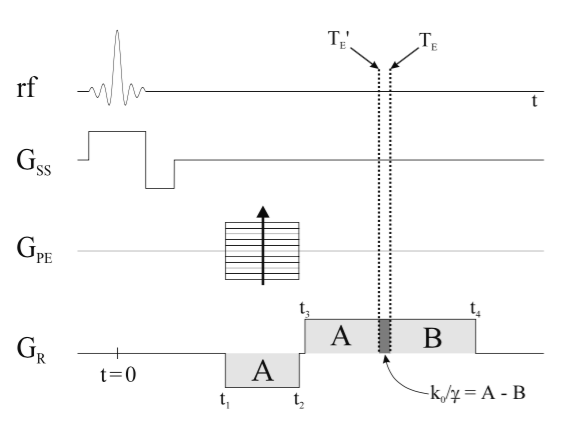
\includegraphics[width=.7\textwidth,keepaspectratio]{fig112}
    \caption{Example of a read gradient structure leading to a shift of the echo in the sampling window. The area under the gradient between $t_1$ and $t_2$ is $A$ and the area under the read gradient itself is $2B$. The echo is shifted from $TE$ to $TE' < TE$ if $A$ is chosen to be less than $B$. This results in a shift of $k_0 < 0$ in the read direction k-space variable. \newline \courtesy}
    \label{fig:fig112}
\end{figure}

%
\subsubsection{Phase Imaging and Phase Aliasing}

\begin{itemize}
    \item Phase imaging is a technique used in MRI where images of the accumulated phase are constructed instead of the classic anatomical or functional ones. Phase images are calculated with the inverse tangent as presented here:
    \begin{flalign*}
        \phi(x,y) \equiv Arg \ \hat{\rho}(x,y) = tan^{-1} \Bigg( \frac{Im \  \hat{\rho}(x,y)}{Re \ \hat{\rho}(x,y)} \Bigg)
    \end{flalign*}
    One particular usefulness is to see whether the expected gradient echo is uncentered. 

    \item Phase Imaging artifact (see Figure~\ref{fig:fig113}):
    \begin{itemize}
        \item \textit{Zebra stripes} are a phase imaging artifact that can be caused by an \textbf{asymmetry in the echo position}. Because of the inverse tangent’s periodicity, spins with phase values differing by multiples of $2\pi$ will have the same intensity and this will cause the aforementioned artifact.

        \item How? 
        The centre of the sampling window is expected to be at $k = 0$, for which the readout gradient phase for all spins is $0$. When this is no longer true, and a certain shift of $k_0$ has happened in the way data was sampled, the measured signal $s_m(k)$ is no longer the true (expected) $s(k)$. Instead, $s_m(k) = s(k-k_0)$.

        \item Applying the shift theorem here yields a reconstructed image in x-space that will also have an additional phase $\Delta \phi(x) = 2\pi k_0 x$.
    \end{itemize}

    \item Besides the gradient echo asymmetry, local field inhomogeneities also cause changes in the phase images.

\end{itemize}

\begin{figure}[H]
    \centering
    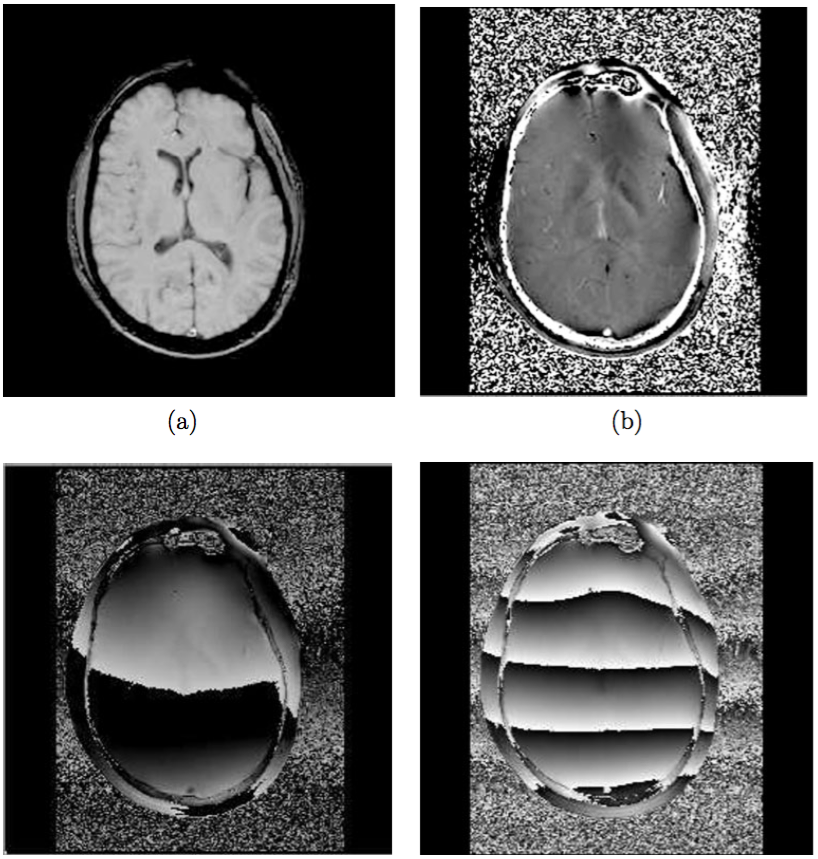
\includegraphics[width=.7\textwidth,keepaspectratio]{fig113}
    \caption{(a) A 2D gradient echo magnitude image of the head. (b) The corresponding phase image of the head when the echo is centered in the read data acquisition window. (c) A phase image taken from the same data that produced (b) except that the echo is shifted 'one sample point' away from the center of the sampling window. (d) A phase image where the echo is shifted five points away from the center of the sampling window. The restricted variation of the phase from $−\pi$ to $\pi$ creates the banding referred to as the 'zebra stripe' artifact. The phase shift occurs along the read (vertical) direction, and the bands are perpendicular to this direction. This is an example of how knowledge of the theory behind an artifact gives information about the sequence acquisition. \newline \courtesy}
    \label{fig:fig113}
\end{figure}

%
\subsubsection{The Duality Theorem}

\begin{itemize}
    \item The Duality Theorem states that if $h(x)$ and $H(k)$ are Fourier transform pairs, then $H(-x)$ and $h(k)$ are also Fourier transform pairs.

    \item Why this is important? 
    \begin{itemize}
        \item Knowing one pair of Fourier transforms will lead to knowing a different pair without any other calculations.
        
        \item Explanation from \href{https://ocw.mit.edu/resources/res-6-007-signals-and-systems-spring-2011/lecture-notes/MITRES_6_007S11_lec09.pdf}{here}: \\
        
            \begin{mdframed}[backgroundcolor=lightgray!20] 
                Duality between the time and frequency domains is another important
                property of Fourier transforms.
                This property relates to the fact that the analysis equation and synthesis equation look almost identical except for a factor
                of $1/2\pi$ and the difference of a minus sign in the exponential in the integral. 
                As a consequence, if we know the Fourier transform of a specified time function, then we also know the Fourier transform of a signal whose functional form is the same as the form of this Fourier transform. 
                Said another way, \textit{the Fourier
                transform of the Fourier transform is proportional to the original signal reversed
                in time}. 
                One consequence of this is that whenever we evaluate one
                transform pair we have another one for free.
                As another consequence, if we
                have an effective and efficient algorithm or procedure for implementing or
                calculating the Fourier transform of a signal, then exactly the same procedure
                with only minor modification can be used to implement the inverse Fourier
                transform. This is, in fact, very heavily exploited in discrete-time signal analysis
                and processing, where explicit computation of the Fourier transform and
                its inverse play an important role.
                [Quotation courtesy of \href{https://ocw.mit.edu/resources/res-6-007-signals-and-systems-spring-2011/lecture-notes/MITRES_6_007S11_lec09.pdf}{MIT}]
            \end{mdframed}
    
    \end{itemize}
    
    \item Deriving the duality theorem \label{proof:duality} (if $h(x) \xLeftrightarrow{\mathfrak{F}} H(k)$, then $H(-x) \xLeftrightarrow{\mathfrak{F}} h(k)$):
    % H(k) \equiv \mathfrak{F}(h(x)) & = \int_{- \infty}^{+ \infty} dx \ h(x) e^{-i 2 \pi kx} \\ 
    \begin{flalign*}
        \text{1) Starting from: } h(x) & = \int_{- \infty}^{+ \infty} dk \ H(k) e^{+i 2 \pi kx} \\
        \text{Change of variable } k & \rightarrow -k \\
        h(x) & = \int_{- \infty}^{+ \infty} dk \ H(-k) e^{-i 2 \pi kx} = \mathfrak{F}(H(-k)) \\
        \text{Change of variable } k & \rightarrow x \\
        h(k) & = \int_{- \infty}^{+ \infty} dx \ H(-x) e^{-i 2 \pi kx} = \mathfrak{F}(H(-x)) 
    \end{flalign*}
    
    \begin{flalign*}
        \text{2) Starting from: } H(k) & = \int_{- \infty}^{+ \infty} dx \ h(x) e^{-i 2 \pi kx} \\ 
        \text{Change of variable } k & \rightarrow -k \\
        H(-k) & = \int_{- \infty}^{+ \infty} dx \ h(x) e^{+i 2 \pi kx} = \mathfrak{F}^{-1}(h(x))\\ 
        \text{Change of variable } k & \rightarrow x \\
        H(-x) & = \int_{- \infty}^{+ \infty} dk \ h(k) e^{+i 2 \pi kx} = \mathfrak{F}^{-1}(h(k))
    \end{flalign*}
    
    \item Duality theorem for shifted Delta function ($\delta(x) \rightarrow \delta(x − x_0)$):
    \begin{flalign*}
        h(x) = \delta(x-x_0) & \xLeftrightarrow{\mathfrak{F}} H(k) = e^{−i2 \pi k x_0} \\
        & \text{and}  \\
        H(-x) = e^{+i2 \pi k x_0} & \xLeftrightarrow{\mathfrak{F}} h(k) = \delta(k-k_0)
    \end{flalign*}
    The shifted Delta function gives rise to a periodic transform with period $1/x_0$ as seen in Figure~\ref{fig:fig1124a}.
    
    \item A classic Fourier transform pair for MRI can be seen in both Figure~\ref{fig:fig1124b} and Figure~\ref{fig:fig1124bBook}, for the $rect(\frac{x}{W}) \xLeftrightarrow{\mathfrak{F}} W \ sinc(\pi Wk)$.

\end{itemize}

\begin{figure}[H]
    \centering
    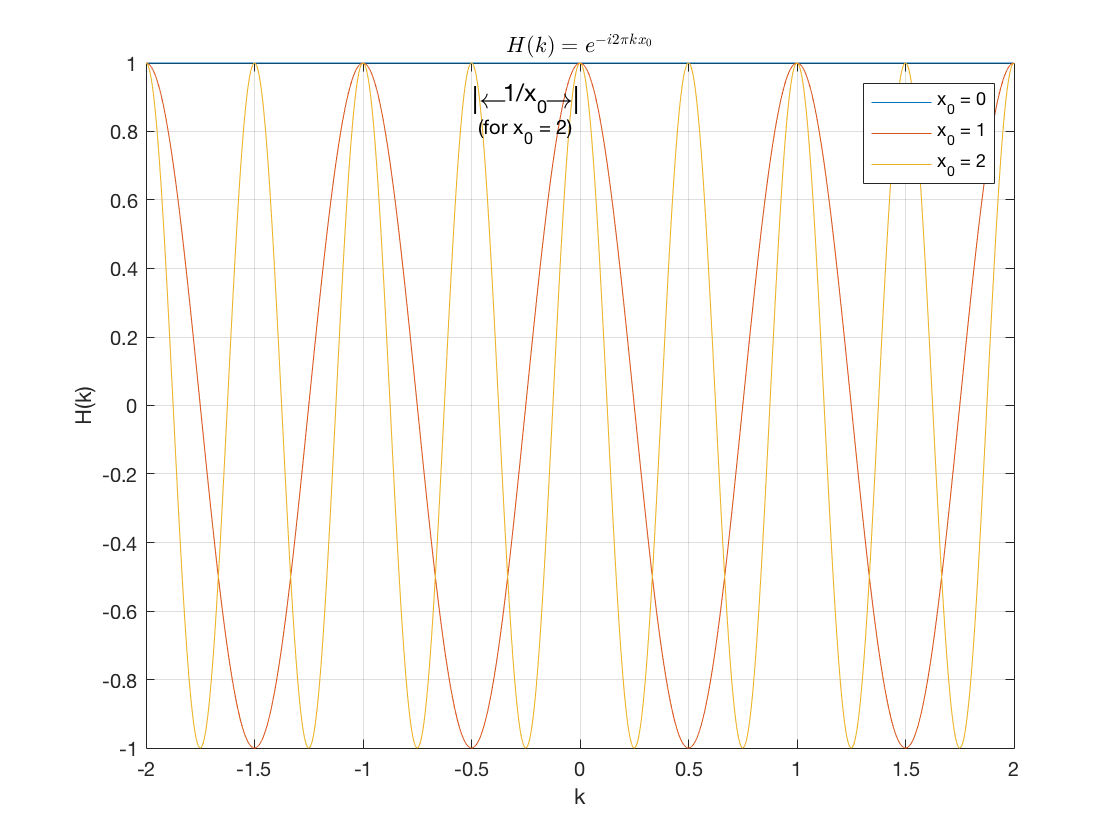
\includegraphics[width=.9\textwidth,keepaspectratio]{fig1124a}
    \caption{The Fourier transform of a shifted Delta function ($H(k) \equiv \mathfrak{F}(\delta(x-x_0)) = e^{-i 2 \pi k x_0}$) is a periodic function (with period $1/x_0$)}
    \label{fig:fig1124a}
\end{figure}

\begin{figure}[H]
    \centering
    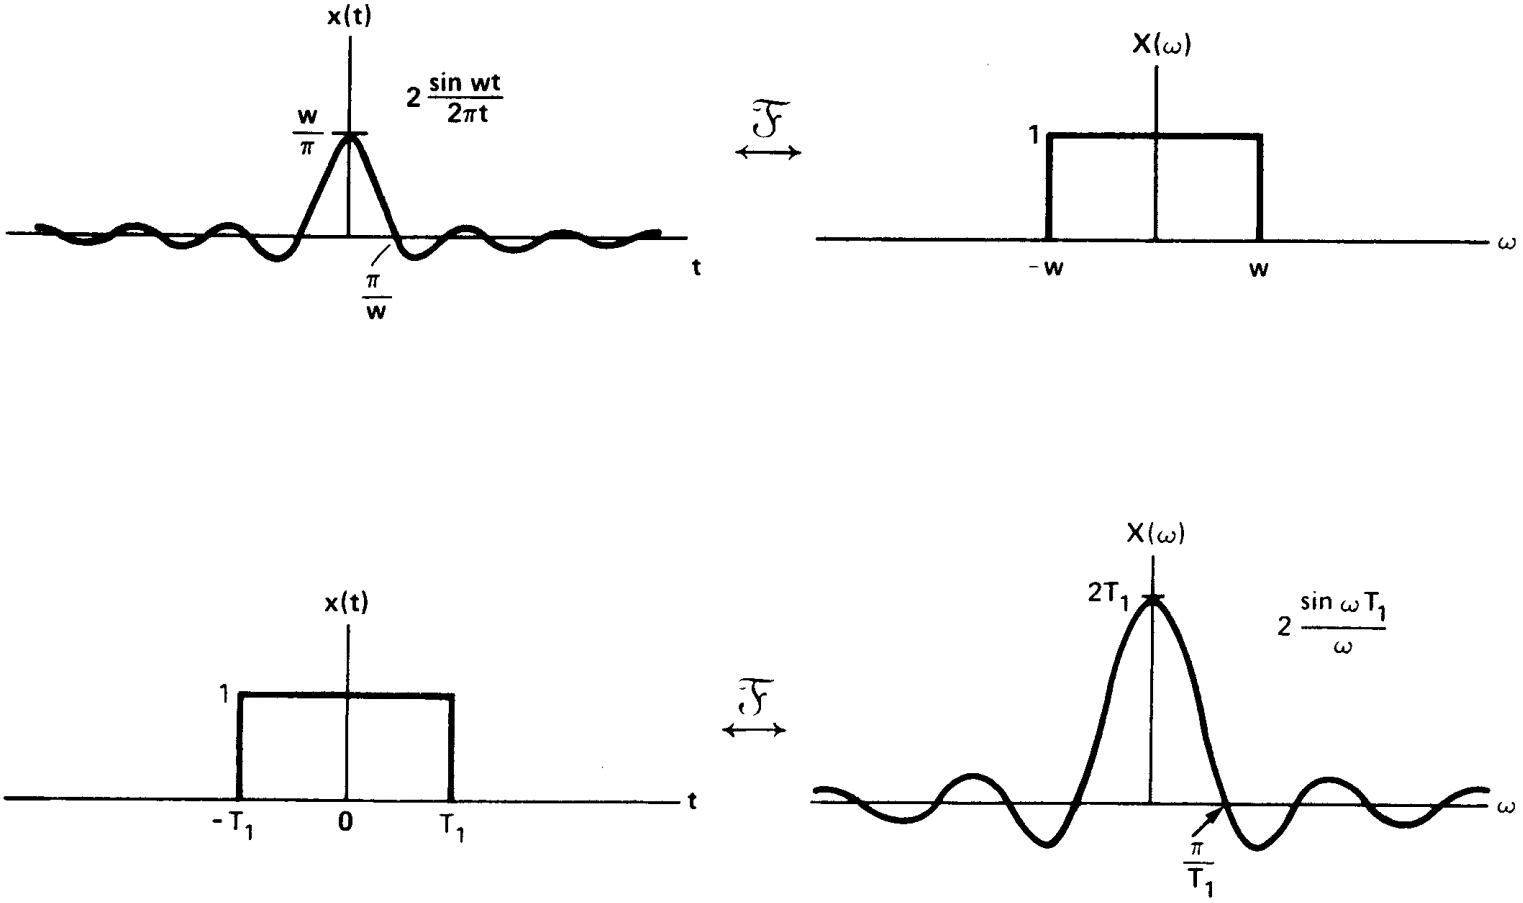
\includegraphics[width=.9\textwidth,keepaspectratio]{fig1124bBook}
    \caption{The $rect(\frac{x}{W}) \xLeftrightarrow{\mathfrak{F}} W \ sinc(\pi Wk)$ Fourier transform pair. 
    Image courtesy of \href{https://ocw.mit.edu/resources/res-6-007-signals-and-systems-spring-2011/lecture-notes/MITRES_6_007S11_lec09.pdf}{MIT} }
    \label{fig:fig1124bBook}
\end{figure}

\begin{figure}[H]
    \centering
    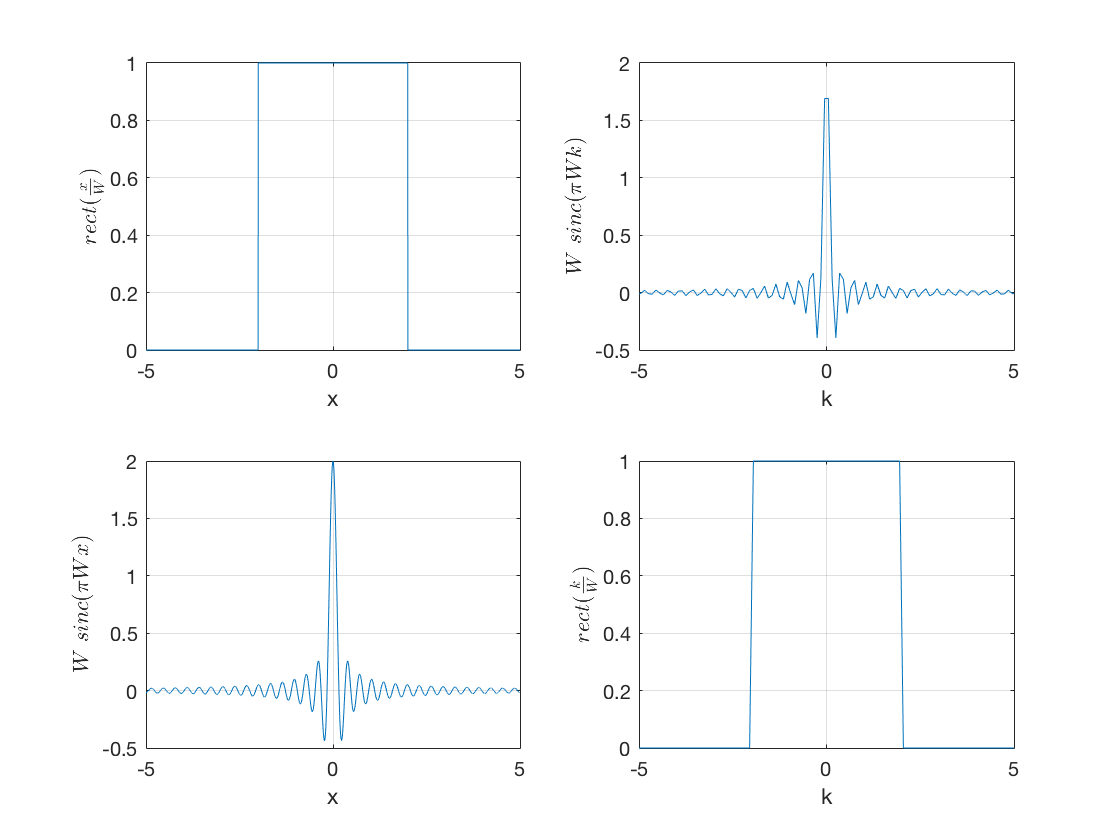
\includegraphics[width=.9\textwidth,keepaspectratio]{fig1124b}
    \caption{The $rect(\frac{x}{W}) \xLeftrightarrow{\mathfrak{F}} W \ sinc(\pi Wk)$ Fourier transform pair}
    \label{fig:fig1124b}
\end{figure}


%
\subsubsection{The Convolution Theorem}
\begin{itemize}
    \item The Convolution Theorem shows that the Fourier transform of the product of two functions is the convolution between the Fourier Transforms of each individual function.
    
    \begin{flalign*}
        \mathfrak{F}(g(x) \cdot h(x)) & = G(k) \ast H(k) \\        
        \text{where: } G(k) \ast H(k) & \equiv \int_{- \infty}^{+ \infty} dk' G(k')H(k − k')
    \end{flalign*}

    \item One example of why this is important to know is that, in MRI, the measured signal can be modelled as a multiplication between the ideal non-decaying signal $s(k)$ and a $T_2^*$ decaying factor. The inverse Fourier transform of this product will yield a convolution between the spin density function and the Fourier transform of the decaying factor.
    
    \item The integral involved in the convolution operation shows that 
    \begin{mdframed}[backgroundcolor=lightgray!20] 
    Finding the convolution of two functions at the position
    x involves reflecting one function through the origin, displacing it by x, and finding the area of the product of the two functions. A graphical representation is useful for a qualitative, and sometimes quantitative, understanding of convolution.
    \courtesyText
    \end{mdframed} 
    The graphical representation is found in Figure~\ref{fig:fig114}.
    
    \item The convolution theorem and Parseval's theorem are found in the Problems section.

\end{itemize}

\begin{figure}[H]
  \begin{center}
    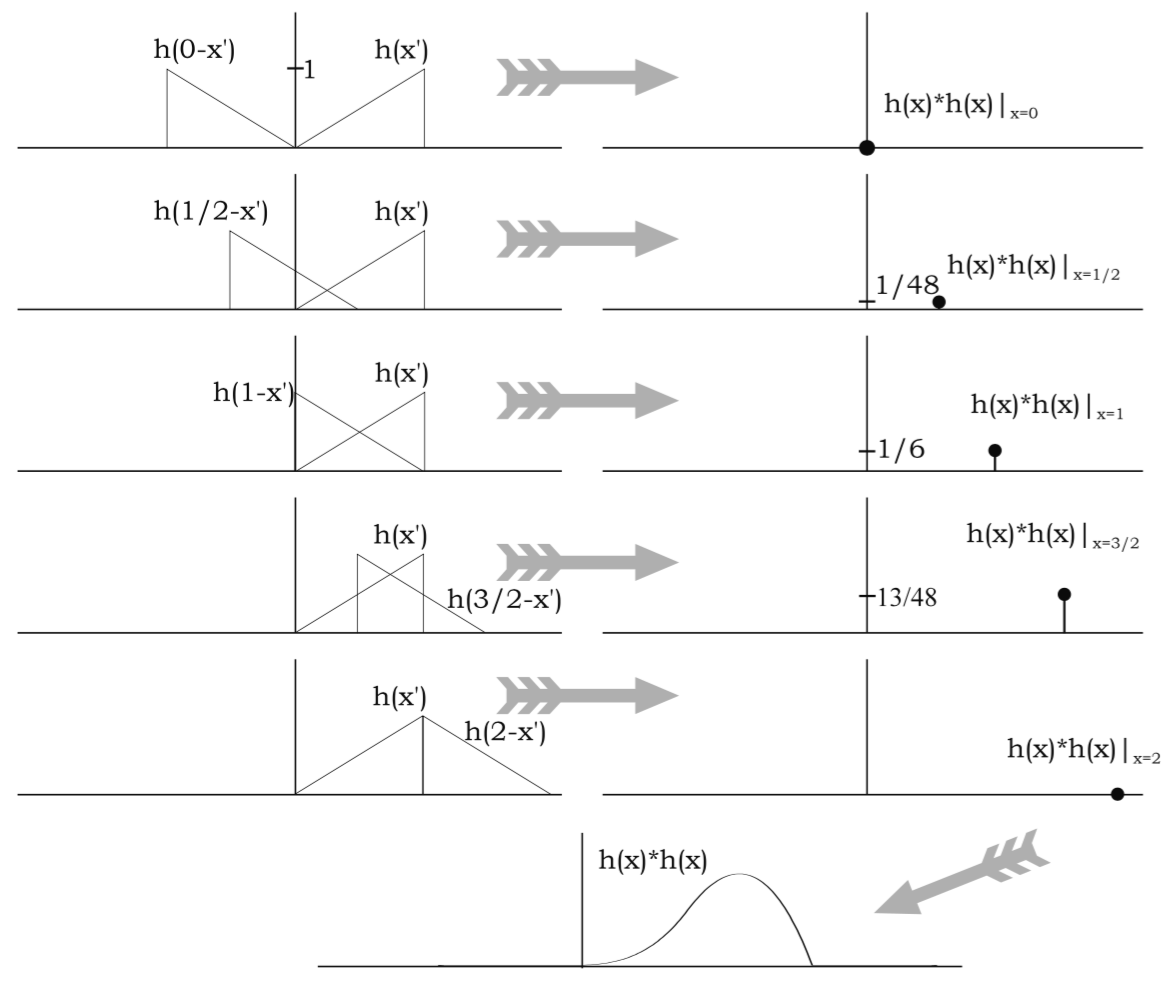
\includegraphics[width=0.8\textwidth,keepaspectratio]{fig114}
  \end{center}
  \caption{A combined graphical and numerical example in convolution. The convolution of a ramp function with itself involves an integration over the product (which is not shown) of the mirror-reflected ramp functions $h(x')$ and $h(x − x')$ both of which are plotted for five different $x$ values. \courtesy}
  \label{fig:fig114}
\end{figure}

%\begin{wrapfigure}{l}{0.5\textwidth}
\begin{figure}
  \begin{center}
    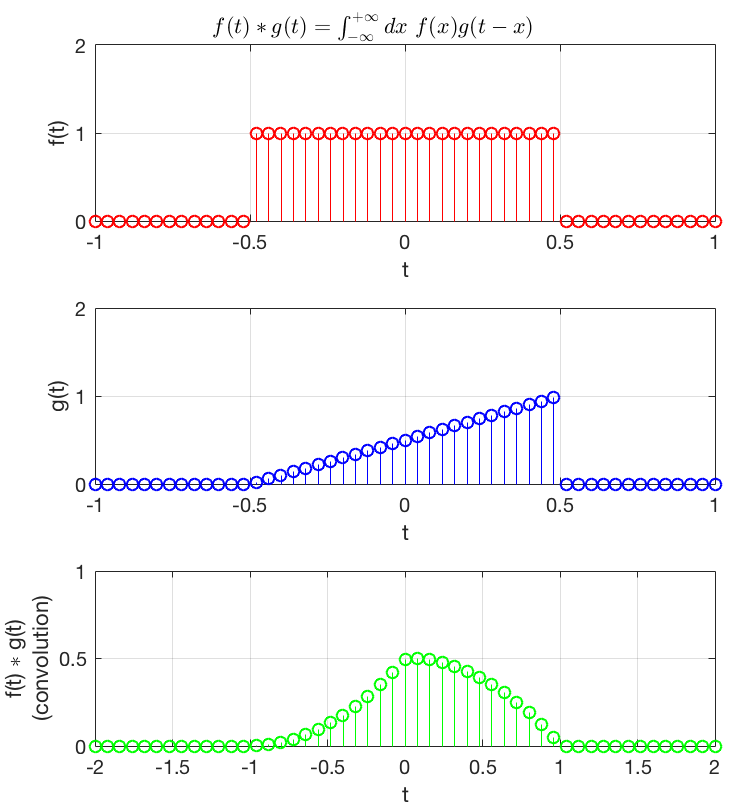
\includegraphics[width=0.48\textwidth,keepaspectratio]{fig1125myconv}
  \end{center}
  \caption{The convolution between a ramp function and a rect function}
  \label{fig:fig1125myconv}
\end{figure}

%
\subsubsection{Convolution Associativity}
\begin{itemize}
    \item Convolution is commutative and associative.
    \begin{flalign*}
        a(x) \ast b(x) &= b(x) \ast a(x) \text{ (\textit{commutativity})} \\
        [a(x) \ast b(x)] \ast c(x) &= a(x) \ast [b(x) \ast c(x)] \text{ (\textit{associativity})}
    \end{flalign*}

    \item These properties are important because later on we shall see that finite sampling and truncation of the signal can be written as a convolution between the ideal signal $s(k)$, a sampling function and a truncation function. The order in which this is done does not matter.
 
\end{itemize}

%
\subsubsection{Derivative Theorem}
\begin{itemize}
    %TODO: Example with a gaussian
    % 0. Add plots from here: http://campar.in.tum.de/Chair/HaukeHeibelGaussianDerivatives 
    % 1. Fourier transform of a gaussian from here: http://www.cse.yorku.ca/~kosta/CompVis_Notes/fourier_transform_Gaussian.pdf
    % 2. Add plot from ch11_2_7.m
    
    \item The derivative theorem states that the Fourier transform of the derivative of a function is the Fourier transform of that function multiplied with $i 2\pi k$
    \begin{flalign*}
        \mathfrak{F}\bigg[\frac{dh}{dx}\bigg] = i 2 \pi k H(k)
    \end{flalign*}

    \item This is an interesting result, as a boundary image can be extracted easily by taking the inverse Fourier transform of the product between the signal $s(k)$ and $i 2 \pi k$.
    
    \item Also,
    \begin{mdframed}
    upon multiplication by $k$, the measured signal, $s_m(k) + \eta_m(k)$, is enhanced at large $k$ values, where noise is relatively more important.
    \courtesyText
    \end{mdframed}
\end{itemize}

\begin{figure}
  \begin{center}
    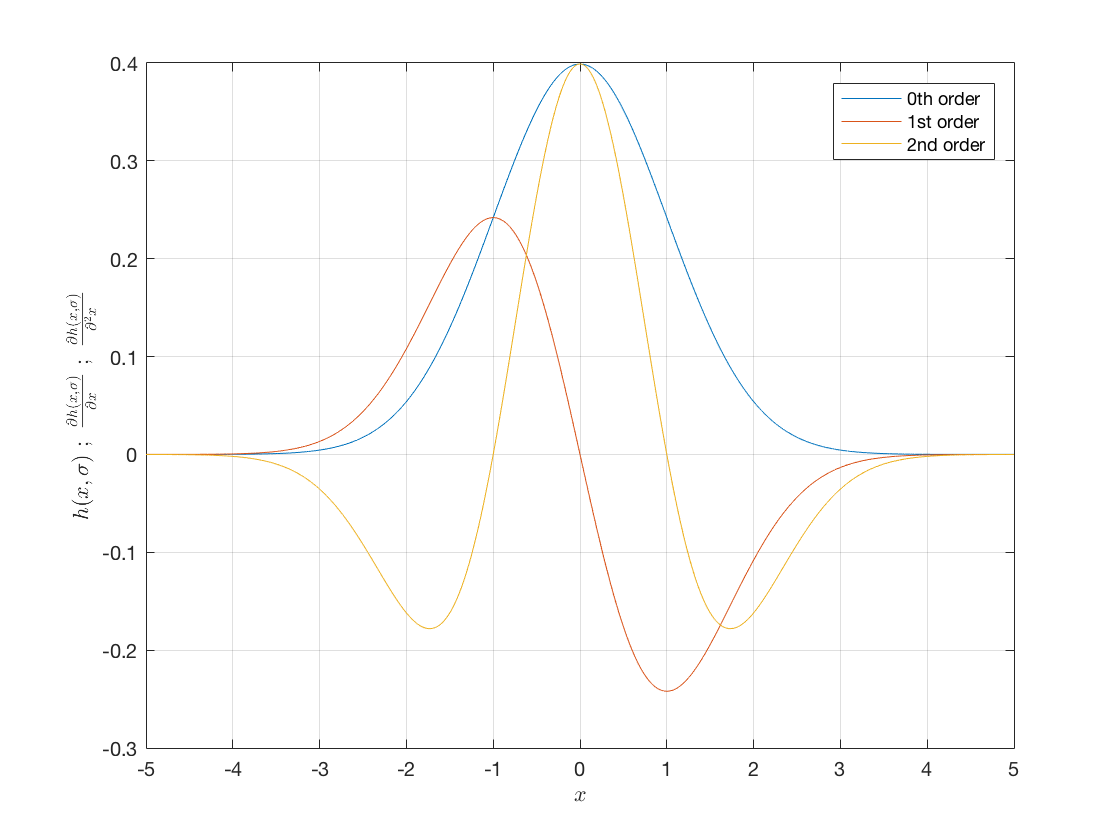
\includegraphics[width=0.8\textwidth,keepaspectratio]{fig1127gauss}
  \end{center}
  \caption{The 0th, 1st and 2nd order 1D Gaussian}
  \label{fig:fig1127gauss}
\end{figure}

\begin{figure}
  \begin{center}
    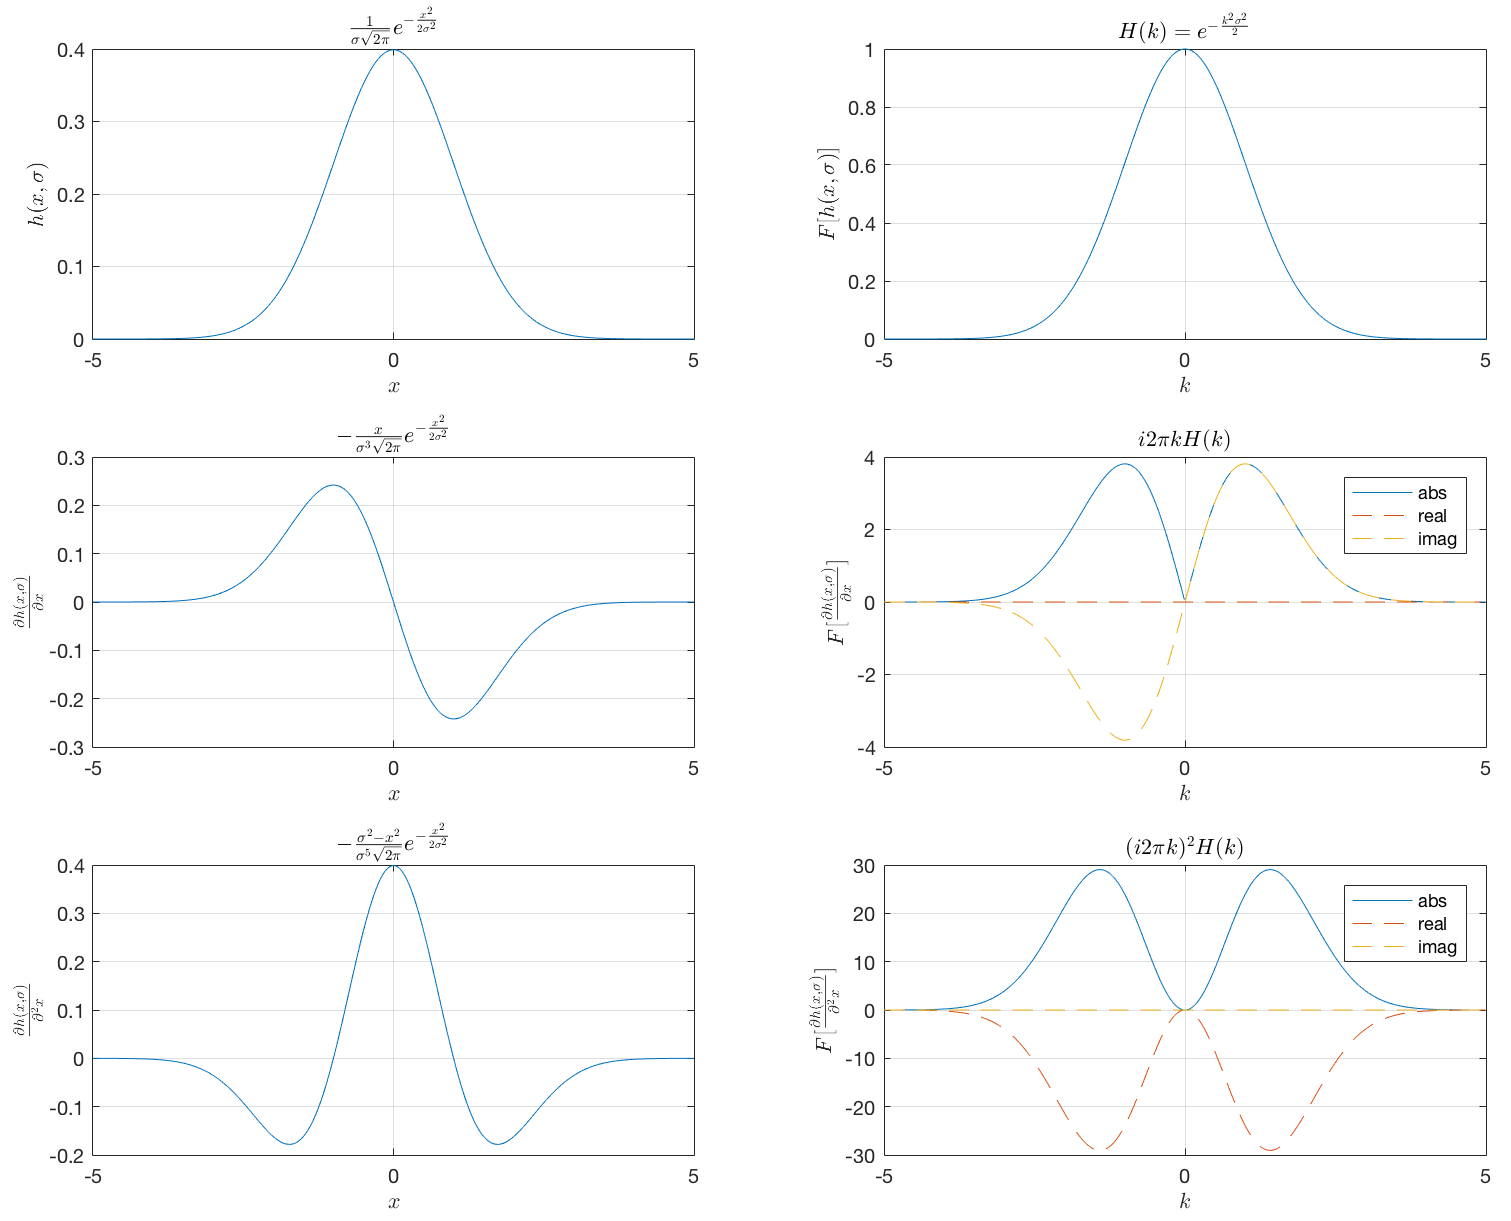
\includegraphics[width=1\textwidth,keepaspectratio]{fig1127gaussfourier}
  \end{center}
  \caption{The Derivative Theorem shown for a 1D Gaussian}
  \label{fig:fig1127gaussfourier}
\end{figure}


\subsubsection{Fourier Transform Symmetries}
\begin{itemize}
    \item The Fourier transform symmetries refers to the symmetry property of a Fourier transform of a real function. More specifically, for $h : \mathfrak{R} \rightarrow \mathfrak{R}$, and $H(k) \equiv \mathfrak{F}(h(x))$, we have: 
    \begin{flalign*}
        Re[H(k)] &= \ \ Re[H(-k)] \text{ \textit{(even symmetry)} and } \\
        Im[H(k)] &= -Im[H(-k)] \text{ \textit{(odd symmetry)}}
    \end{flalign*}
    
    \item A useful consequence of this property is seen in \textit{partial Fourier imaging}. This technique takes advantage of the complex conjugate symmetry ($H(k) = H^*(-k)$) of the k-space data for purely real spin density functions. This means that you can acquire half of k-space and generate the missing quantities by assuming conjugate symmetry.
    
    \item This property also tells us that the Fourier transform of an even/odd function will also be an even/odd function. Let's test this with the cosine and sine functions:
    
    \begin{flalign*}
        1) \ C(k) & = \mathfrak{F}[cos(2 \pi k_0 x)] = \\
        & = \int_{- \infty}^{+ \infty} dx \ cos(2 \pi k_0 x) e^{-i 2 \pi k x} \\
        & = \int_{- \infty}^{+ \infty} dx \ \frac{e^{i2 \pi k_0 x} + e^{-i2 \pi k_0 x}}{2} e^{-i 2 \pi k x} \\
        & = \frac{1}{2} \int_{- \infty}^{+ \infty} dx \ e^{-i2 \pi (k-k_0) x} + \frac{1}{2} \int_{- \infty}^{+ \infty} dx \ e^{-i2 \pi (k+k_0) x}\\
        & = \frac{1}{2} \delta(k-k_0) + \frac{1}{2} \delta(k+k_0) \\
        C(-k) & = \frac{1}{2} \delta(-(k+k_0)) + \frac{1}{2} \delta(-(k-k_0)) \\
        & = \frac{1}{2} \delta(k+k_0) + \frac{1}{2} \delta(k-k_0) = C(k) \\
    \end{flalign*}
    
    \begin{flalign*}
        2) \ S(k) & = \mathfrak{F}[sin(2 \pi k_0 x)] = \\
        & = \int_{- \infty}^{+ \infty} dx \ sin(2 \pi k_0 x) e^{-i 2 \pi k x} \\
        & = \int_{- \infty}^{+ \infty} dx \ \frac{e^{i2 \pi k_0 x} - e^{-i2 \pi k_0 x}}{2i} e^{-i 2 \pi k x} \\
        & = \frac{1}{2i} \int_{- \infty}^{+ \infty} dx \ e^{-i2 \pi (k-k_0) x} - \frac{1}{2i} \int_{- \infty}^{+ \infty} dx \ e^{-i2 \pi (k+k_0) x}\\
        & = \frac{i}{2} \delta(k+k_0) - \frac{i}{2} \delta(k-k_0) \\
        S(-k) & = -\frac{i}{2} \delta(-(k+k_0)) + \frac{i}{2} \delta(-(k-k_0)) \\
        & = -\frac{i}{2} \delta(k+k_0) + \frac{i}{2} \delta(k-k_0) = -S(k)
    \end{flalign*}
    
    \textcolor{gray}{\textbf{Sidenote}: 
    \begin{flalign*}
        e^{ix} &= cos(x) + i sin(x) \\
        e^{-ix} &= cos(x) - i sin(x) \\
        e^{ix} + e^{-ix} &= 2 cos(x) \Rightarrow cos(x) = \frac{e^{ix} + e^{-ix}}{2} \\
        e^{ix} - e^{-ix} &= 2i \ sin(x) \Rightarrow sin(x) = \frac{e^{ix} - e^{-ix}}{2i}
    \end{flalign*}}
\end{itemize}

\begin{figure}
  \begin{center}
    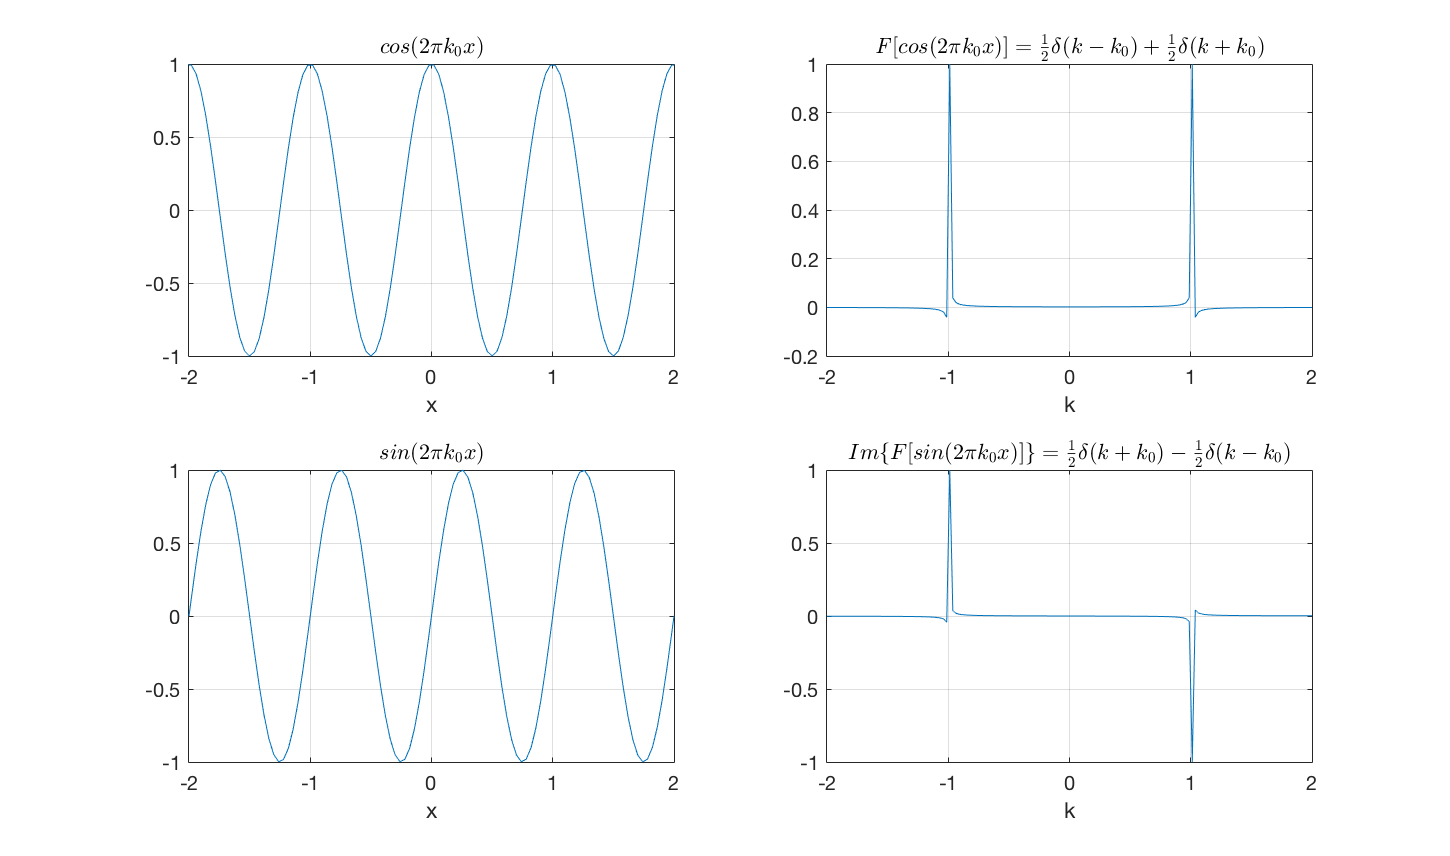
\includegraphics[width=1\textwidth,keepaspectratio]{fig1128}
  \end{center}
  \caption{The odd/even behaviour of sin/cos}
  \label{fig:fig1128}
\end{figure}

\clearpage
%
\subsubsection{Summary of the mathematical properties of the continuous Fourier transform}
% \begin{table}[h!]
% \centering
\begin{longtable}{l l l} 
 \hline
 \textbf{Property} & \textbf{Mathematical Expression} & \textbf{Proof} \\ 
 \hline\hline
 
 linearity 
 & $\mathfrak{F}[\alpha h(x)] = \alpha \mathfrak{F}[h(x)]$ 
 & \begin{tabular}{@{}l@{}}$\mathfrak{F}[\alpha h(x)] =$ \\ $= \int_{- \infty}^{+ \infty} dx \ \alpha h(x) e^{-i 2 \pi k x}$ \\ $= \alpha \int_{- \infty}^{+ \infty} dx \ h(x) e^{-i 2 \pi k x}$ \\ $= \alpha \mathfrak{F}(h(x)) $\end{tabular} \\ 
 
 \hline
 
 " 
 & \begin{tabular}{@{}l@{}} $\mathfrak{F}[h_1(x) + h_2(x)] =$ 
 \\ $\mathfrak{F}[h_1(x)] + \mathfrak{F}[h_2(x)]$  \end{tabular}
 & \begin{tabular}{@{}l@{}} $\mathfrak{F}[h_1(x) + h_2(x)] = $ 
 \\ $= \int_{- \infty}^{+ \infty} dx \ (h_1(x) + h_2(x)) e^{-i 2 \pi k x}$ 
 \\ $= \int_{- \infty}^{+ \infty} dx \ h_1(x) e^{-i 2 \pi k x} + \int_{- \infty}^{+ \infty} dx \ h_2(x) e^{-i 2 \pi k x}$ 
 \\ $= \mathfrak{F}(h_1(x)) + \mathfrak{F}(h_2(x))$ \end{tabular} \\
 
 \hline
 
 duality 
 & \begin{tabular}{@{}l@{}} if $h(x) \xLeftrightarrow{\mathfrak{F}} H(k)$ 
 \\ then $H(-x) \xLeftrightarrow{\mathfrak{F}} h(k)$ \end{tabular} 
 & Proof in Section \ref{proof:duality} \\
 
 \hline
 
 \begin{tabular}{@{}l@{}} space \\ scaling \end{tabular}
 & $\mathfrak{F}(h(\alpha x)) = \frac{1}{\lvert a \rvert} H(\frac{k}{\alpha})$ 
 & TBA \\
 
 \hline
 
 \begin{tabular}{@{}l@{}} space \\ shifting \end{tabular}
 & $\mathfrak{F}(h(x \pm x_0)) = H(k) e^{\pm i2 \pi k x_0}$ 
 & \begin{tabular}{@{}l@{}} $\mathfrak{F}(h(x-x_0)) = $ 
 \\ $= \int_{- \infty}^{+ \infty} dx \ h(x-x_0) e^{-i 2 \pi k x}$
 \\ Change of variable: $x' = x-x_0$ 
 \\ $= e^{-i 2 \pi k x_0} \ \int_{- \infty}^{+ \infty} dx' \ h(x') e^{-i 2 \pi k x'}$ 
 \\ $= e^{-i 2 \pi k x_0} \ H(k)$ \end{tabular} \\
 
 \hline
 
 \begin{tabular}{@{}l@{}} frequency \\ shifting \end{tabular}
 & $\mathfrak{F}^{-1}(H(k \pm k_0)) = h(x) e^{\mp i2 \pi k_0 x}$ 
 & \begin{tabular}{@{}l@{}} $\mathfrak{F}^{-1}(H(k - k_0)) = $ 
 \\ $= \int_{- \infty}^{+ \infty} dk \ H(k-k_0) e^{+i 2 \pi k x}$
 \\ Change of variable: $k' = k-k_0$ 
 \\ $= e^{+i 2 \pi k_0 x} \ \int_{- \infty}^{+ \infty} dk' \ H(k') e^{-i 2 \pi k' x}$ 
 \\ $= e^{+i 2 \pi k_0 x} \ h(x)$ \end{tabular} \\
 
 \hline
 
 \begin{tabular}{@{}l@{}} alternate \\ form \end{tabular}
 & $h^*(x) = \mathfrak{F}^{-1}[H^*(-k)]$ 
 & \begin{tabular}{@{}l@{}} $h(x) = \int_{- \infty}^{+ \infty} dk H(k) e^{+ i 2 \pi kx} \Rightarrow$ 
 \\ $[h(x)]^* = [\int_{- \infty}^{+ \infty} dk \ H(k) e^{+ i 2 \pi kx}]^* \Rightarrow$ 
 \\ $h^*(x) = \int_{- \infty}^{+ \infty} dk \ H^*(k) e^{- i 2 \pi kx} \Rightarrow$
 \\ Change of variable $k = -k \Rightarrow$
 \\ $h^*(x) = \int_{- \infty}^{+ \infty} dk \ H^*(-k) e^{+ i 2 \pi kx} \Rightarrow$
 \\ $h^*(x) = \mathfrak{F}^{-1}[H^*(-k)]$
 \end{tabular} \\
 
 \hline
 
 even $h(x)$
 & $H(k) = 2 \int_{0}^{+ \infty} dx \ h(x) \ cos( 2\pi k x)$ 
 & \begin{tabular}{@{}l@{}} $H(k) = \int_{- \infty}^{+ \infty} dx \ h(x) \ e^{- i 2 \pi k x}$ 
 \\ $= \int_{- \infty}^{0} dx \ h(x) \ e^{- i 2 \pi k x} + \int_{0}^{+\infty} dx \ h(x) \ e^{- i 2 \pi k x} $
 \\ Because $h(x) = h(-x) \Rightarrow$
 \\ $= \int_{0}^{+ \infty} dx \ h(x) \ e^{+ i 2 \pi k x} + \int_{0}^{+\infty} dx \ h(x) \ e^{- i 2 \pi k x} $
 \\ $= \int_{0}^{+ \infty} dx \ h(x) \ (e^{+ i 2 \pi k x}+e^{- i 2 \pi k x})$
 \\ $= 2 \ \int_{0}^{+ \infty} dx \ h(x) \ cos(2 \pi k x)$
 \end{tabular} \\
 
 \hline
 
 odd $h(x)$
 & $H(k) = -2i \int_{0}^{+ \infty} dx \ h(x) \ sin( 2\pi k x)$ 
 & \begin{tabular}{@{}l@{}} $H(k) = \int_{- \infty}^{+ \infty} dx \ h(x) \ e^{- i 2 \pi k x}$ 
 \\ $= \int_{- \infty}^{0} dx \ h(x) \ e^{- i 2 \pi k x} + \int_{0}^{+\infty} dx \ h(x) \ e^{- i 2 \pi k x} $
 \\ Because $-h(x) = h(-x) \Rightarrow$
 \\ $= -\int_{0}^{+ \infty} dx \ h(x) \ e^{+ i 2 \pi k x} + \int_{0}^{+\infty} dx \ h(x) \ e^{- i 2 \pi k x} $
 \\ $= \int_{0}^{+ \infty} dx \ h(x) \ (-e^{+ i 2 \pi k x}+e^{- i 2 \pi k x})$
 \\ $= -2i \ \int_{0}^{+ \infty} dx \ h(x) \ sin(2 \pi k x)$
 \end{tabular} \\
 
 \hline
 
 convolution
 & \begin{tabular}{@{}l@{}} $\mathfrak{F}[g(x)h(x)]$ 
 \\ $= G(k) \ast H(k)$ 
 \\ $\equiv \int_{- \infty}^{+ \infty} dk' G(k')H(k-k')$ \end{tabular}
 & Proof in Section \ref{proof:convolution} \\
 
 \hline
 
 derivative
 & $\mathfrak{F}[\frac{dh}{dx}] = i 2 \pi k H(k)$
 & \begin{tabular}{@{}l@{}} $h(x) = \int_{- \infty}^{+ \infty} dk \ H(k) e^{+ i 2 \pi k x} \Rightarrow$ 
 \\ $[h(x)]' = [\int_{- \infty}^{+ \infty} dk \ H(k) e^{+ i 2 \pi k x}]'  \Rightarrow$
 \\ $\frac{d h}{dx} = \int_{- \infty}^{+ \infty} dk \ H(k) \ \frac{d}{dx} e^{+ i 2 \pi k x}  \Rightarrow$
 \\ $\frac{d h}{dx} = i 2 \pi k \ \int_{- \infty}^{+ \infty} dk \ H(k) e^{+ i 2 \pi k x}  \Rightarrow$ 
 \\ $\frac{d h}{dx} = i 2 \pi k \ h(x)  \Rightarrow$ 
 \\ $\mathfrak{F}[\frac{d h}{dx}] = i 2 \pi k \ \mathfrak{F}[h(x)] $ 
 \\ $\mathfrak{F}[\frac{d h}{dx}] = i 2 \pi k \ H(k) $ 
 \end{tabular} \\
 
  \hline
 
 Parseval
 & $ \int_{- \infty}^{+ \infty} dx \ \lvert g(x) \rvert ^2  = \int_{- \infty}^{\infty} dk \ \lvert G(k)  \rvert ^2$
 & Proof in Section \ref{proof:parseval} \\
 
 
 %\begin{tabular}{@{}l@{}} \end{tabular}
 \hline
\caption{Important mathematical properties of the continuous Fourier transform}
\label{table:1}
\end{longtable}

% \caption{Important mathematical properties of the continuous Fourier transform}
% \label{table:1}
% \end{table}


\clearpage
%%
\subsection{Fourier Transform Pairs}

\subsubsection{The rect and sinc function}
\begin{flalign*}
    & \text{The rectangular function } h(x) = rect \Big( \frac{x}{W} \Big) \text{ has the following Fourier transform pair: } H(k) = W sinc(\pi k W) \\
    & \text{\textit{Proof:}}
\end{flalign*}
\begin{flalign*}
    \text{Let: } h(x) &= rect \Big( \frac{x}{W} \Big) \text{ where: } rect \Big( \frac{x}{W} \Big) \equiv \begin{cases}
               1, \ - \frac{W}{2} \leq x \leq \frac{W}{2} \\
               0, \ \text{otherwise}
            \end{cases}\\
    \text{Then: } H(k) \equiv \mathfrak{F}(h(x)) &= \int_{- \infty}^{+ \infty} dx \ h(x) \ e^{-i 2 \pi k x} \\
    & = \int_{- \infty}^{+ \infty} dx \ rect \Big( \frac{x}{W} \Big) \ e^{-i 2 \pi k x} \\
    & = \int_{- W/2}^{+ W/2} dx \ e^{-i 2 \pi k x}  \\
    & = - \frac{1}{i 2 \pi k} e^{- i 2 \pi k x} \Big\rvert_{-W/2}^{W/2} \\
    & = \frac{1}{i 2 \pi k} \Big( - e^{- i \pi k W} + e^{ i \pi k W} \Big) \\
    \text{Knowing that: } sin(k) &= \frac{e^{ik} - e^{-ik}}{2i} \text{ we get: } \\
    & = \frac{1}{i 2 \pi k} 2 i \ sin(\pi k W) \\
    & = \frac{W}{\pi k W} \ sin(\pi k W) \\
    & = W sinc(\pi k W)
\end{flalign*}
\textcolor{gray}{\textbf{Sidenote}: \\
In x-space, the bigger the $W$, the wider the rectangular function, \\
In k-space, the bigger the $W$, the narrower the sinc function.}

\clearpage
\subsubsection{Gaussian}
\begin{flalign*}
    & \text{The Gaussian function, } g(x) = \frac{1}{\sigma \sqrt{2 \pi}} e^{\frac{-x^2}{2 \sigma^2}} \text{ has the following Fourier transform pair: } G(k) = e^{\frac{-4 \pi^2 \sigma^2 k^2}{2}} \\
    & \text{\textit{Proof:}}
\end{flalign*}
\begin{flalign*}
    g(x) & = \frac{1}{\sigma \sqrt{2 \pi}} e^{\frac{-x^2}{2 \sigma^2}} \ \xRightarrow{\text{differentiate (1)}} \\
    \frac{d g(x)}{dx} & = - \frac{x}{\sigma^3 \sqrt{2 \pi}} \ e^{\frac{-x^2}{2 \sigma^2}} \\
    \frac{d g(x)}{dx} & = - \frac{x}{\sigma^2} \ g(x) \ \xRightarrow{\text{Fourier transform}} \\
    \mathfrak{F}[\frac{d g(x)}{dx} ] & = - \frac{1}{\sigma^2} \ \mathfrak{F}[xg(x)] \xRightarrow{(2)} \\
    i 2 \pi k \ G(k) & = - \frac{1}{\sigma^2} \ \frac{i}{2 \pi} \ \frac{dG(k)}{dk} \\
    \frac{\frac{dG(k)}{dk}}{G(k)} & = - 4 \pi^2 \sigma^2 k \xRightarrow{integrate} \\
    \int_{0}^{k} dk' \ \frac{\frac{dG(k')}{dk'}}{G(k')} & = - 4 \pi^2 \sigma^2 \int_{0}^{k} dk' \  k' \\
    ln \Big( G(k') \Big) \Bigg\rvert_{0}^{k} & = - \frac{4 \pi^2 \sigma^2 k^2}{2} \\
    ln \Big( G(k) \Big) - ln \Big( G(0) \Big)  & = - \frac{4 \pi^2 \sigma^2 k^2}{2} \xRightarrow{G(0) = 1} \\
    ln \Big( G(k) \Big) & = - \frac{4 \pi^2 \sigma^2 k^2}{2} \xRightarrow{\text{apply the exponent}} \\
    e^{ln(G(k))} & = e^{- \frac{4 \pi^2 \sigma^2 k^2}{2}} \\
    G(k) & = e^{- \frac{4 \pi^2 \sigma^2 k^2}{2}}
\end{flalign*}
\textcolor{gray}{\textbf{Sidenote}: \\
(1) $\frac{d}{dx} e^{f(x)} = \frac{df(x)}{dx} \ e^{f(x)}$ \\
(2) $\mathfrak{F}[x g(x)] = \int_{- \infty}^{+ \infty} dx \ xg(x) e^{-i 2 \pi k x} = \int_{- \infty}^{+ \infty} dx \ \frac{i}{2 \pi} \frac{d}{dk} \Big[ g(x) e^{-i 2 \pi k x} \Big] = \frac{i}{2 \pi} \ \frac{d}{dk} \Big[ \int_{- \infty}^{+ \infty} dx \ g(x) e^{-i 2 \pi k x} \Big] = \frac{i}{2 \pi} \frac{dG(k)}{dk} $}

\clearpage
\subsubsection{Lorentzian form}
\begin{flalign*}
    & \text{The Gaussian function, } g(x) = \frac{1}{\sigma \sqrt{2 \pi}} e^{\frac{-x^2}{2 \sigma^2}} \text{ has the following Fourier transform pair: } G(k) = e^{\frac{-4 \pi^2 \sigma^2 k^2}{2}} \\
    & \text{\textit{Proof:}}
\end{flalign*}

\clearpage
\subsubsection{Sampling ('comb') function}

\clearpage
\subsubsection{Fourier transform pairs}
\begin{longtable}{c c c c} 
 \hline
 
 rect function
 & $rect(\frac{x}{W})$ 
 & $\xLeftrightarrow{\mathfrak{F}}$
 & $W sinc(\pi W k)$ \\
 %\begin{tabular}{@{}l@{}}$\mathfrak{F}[\alpha h(x)] =$ \\ $= \int_{- \infty}^{+ \infty} dx \ \alpha h(x) e^{-i 2 \pi k x}$ \\ $= \alpha \int_{- \infty}^{+ \infty} dx \ h(x) e^{-i 2 \pi k x}$ \\ $= \alpha \mathfrak{F}(h(x)) $\end{tabular} \\ 
 
 \hline
 
 Gaussian
 & $rect(\frac{x}{W})$ 
 & $\xLeftrightarrow{\mathfrak{F}}$
 & $W sinc(\pi W k)$ \\
 
 \hline
 
 Lorentzian
 & $rect(\frac{x}{W})$ 
 & $\xLeftrightarrow{\mathfrak{F}}$
 & $W sinc(\pi W k)$ \\
 
 \hline
 
 Sampling ('comb') function
 & $rect(\frac{x}{W})$ 
 & $\xLeftrightarrow{\mathfrak{F}}$
 & $W sinc(\pi W k)$ \\
 
 
 %\begin{tabular}{@{}l@{}} \end{tabular}
 \hline
\caption{Fourier transform pairs important to MRI}
\label{table:2}
\end{longtable}

\clearpage
%%
\subsection{The Discrete Fourier Transform}


\clearpage
%%
\subsection{Discrete Transform Properties}
